\documentclass[a4paper,12pt]{scrartcl}

\usepackage{exercice_sheet}

%\trait
%\section*{}
%\exo{}
%\question{}
%\subquestion{}

\date{}


% Title Page
\title{Fonctions exponentielle et logarithme}

\author{\textsc{Mathématiques}}
\begin{document}

\maketitle

\tableofcontents
  
\section{Fonction exponentielle}

\subsection{Première approche}

\subsubsection{Vocabulaire}

% \begin{center}
% \Huge
% ${x}^{y}$
% \normalsize
% \end{center}

Dans la notation qui suit, $x$ est la \emph{base} et $y$ est l'\emph{exposant}.

\begin{center}
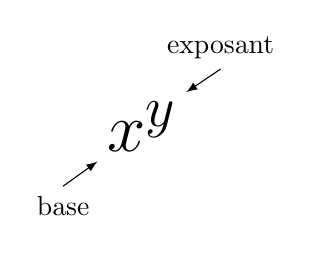
\begin{tikzpicture}
\node (N) at (0,0) {\Huge ${x}^{y}$ \normalsize};
\node (BaseText) at (-1,-1) {base};
\node (ExpoText) at (1,1) {exposant};
\draw[->,>=latex] (BaseText.north) -- (N.south west);
\draw[->,>=latex] (ExpoText.south) -- (N.north east);
\end{tikzpicture}
\end{center}

C'est pour cela qu'on dit que la fonction $e^x$ est la fonction exponentielle de base $e$.

\subsubsection{Définition}

Compléter le tableau suivant à l'aide de la calculatrice ou d'un tableur:

\begin{center}
\begin{tabular}{|l|l|l|l|l|l|l|l|}
\hline
$x$       & -3 & -1 & 0 & 0.5 & 1 & 2 & 5 \\ \hline
$2.718^x$ &  \hspace{3em}  &  \hspace{3em}  & \hspace{3em}  &  \hspace{3em}   & \hspace{3em}  & \hspace{3em}  & \hspace{3em}  \\ \hline
$e^x$       &    &    &   &     &   &   &   \\ \hline
\end{tabular}
\end{center}

Que constate-t-on?

\cadre{1}

\begin{definition}{fonction exponentielle}
 On appelle \og{}fonction exponentielle de base $e$\fg{} ou simplement \og{}fonction exponentielle\fg{}, la fonction définie pour tout $x \in \mathbb{R}$, $f(x) =  e^x$ où $e \approx 2,71828\ldots$ 
\end{definition}

C'est un nombre que l'on rencontre dans de nombreuses applications.

Ensemble de définition: $\mathcal{D}_f = \mathbb{R}$.

On peut également noter $\exp : x \longmapsto e^x$.

\subsubsection{Ensemble de définition}

La fonction exponentielle est définie pour tout nombre réel, autrement dit: 

\Answer{$\mathcal{D}_{\exp} = \mathbb{R}$}

\subsection{Représentation graphique} 

La représentation graphique de la fonction exponentielle est la suivante:

\begin{center}
\simpleplot{-2}{2.5}{\x}{{exp(\x)}}{$e^x$}{1.5}
\end{center}

La fonction exponentielle est strictement croissante sur $\mathbb{R}$. Voici donc son tableau de variation:

\begin{center} 
\begin{tikzpicture}
   \tkzTabInit{$x$ / 1 , $e^x$ / 2}{$-\infty$, $+\infty$}
   \tkzTabVar{-/ $0$, +/ $+\infty$}
\end{tikzpicture} 
\end{center}

De ce fait, on a l'équivalence suivante: $a \geqslant b \Leftrightarrow e^a \geqslant e^b$ (voir la définition d'une fonction croissante).

\subsection{Propriétés}

\subsubsection{Valeurs particulières}

\begin{enumerate}
 \item $e^0 = 1$
 \item $e^1 = e \approx 2.718$ 
\end{enumerate}

\subsubsection{Propriétés opératoires}

Il faut garder en tête que la notation $e^x$ est une puissance, au même titre que par exemple $10^x$ ou $2^x$. La fonction exponentielle a donc les propriétés des fonctions puissance.

\begin{enumerate}
 \item $e^{x+y} = e^x \times e^y$
 \item $e^{x-y} = \dfrac{e^x}{e^y}$
 \item $\left(e^x \right)^y = e^{xy}$. Attention: ne pas confondre $e^{xy}$ et $e^{x^y} = e^{(x^y)}$
 \item $e^{-x} = \dfrac{1}{e^x}$ (découle de la seconde propriété)
 \item pour tout $x \in \mathbb{R}, e^x > 0$. On dit que la fonction exponentielle est \emph{strictement positive} sur $\mathbb{R}$.
\end{enumerate}

Exemple: 

Montrer que $e^{2x-1} = \dfrac{(e^x)^2}{e}$.

\cadre{3}

\subsubsection{Limites}

\begin{equation*}
 \lim_{x \rightarrow -\infty} e^x = \ldots
\end{equation*}

\begin{equation*}
 \lim_{x \rightarrow +\infty} e^x = \ldots
\end{equation*}

\section{Logarithme népérien}

\subsection{Première approche}

\subsubsection{Définition}

Compléter le tableau suivant à l'aide de la calculatrice ou d'un tableur.

\begin{center}
\begin{tabular}{|l|l|l|l|l|l|}
\hline
$x$      & -1 & 0 & 1 & 2 & 4 \\ \hline
$y = e^x$ &  \hspace{3em}  & \hspace{3em}  &  \hspace{3em} &  \hspace{3em} &  \hspace{3em} \\ \hline
$\ln y$   &    &   &   &   &   \\ \hline
\end{tabular}
\end{center}

Que remarque-t-on?

\cadre{2}

Pour tout $x \in \mathbb{R}$, si à $x$ on applique la fonction exponentielle de base $e$ puis la fonction logarithme népérien, on obtient $x$, soit \answer{$\ln(e^x) = x$}.

Pour tout $x > 0$, si à $x$ on applique la fonction logarithme népérien puis la fonction exponentielle de base $e$, on obtient $x$, soit \answer{$e^{\ln x} = x$}.

On dit que la fonction logarithme népérien est la \emph{réciproque} de la fonction exponentielle de base $e$.

% \begin{equation*}
% x \mylongmapsto{\exp(x)} e^x \mylongmapsto{\ln(x)} x
% \end{equation*}
\begin{equation*}
 x \longmapsto e^x \longmapsto x
\end{equation*}

Nous utiliserons cette propriété pour résoudre beaucoup de problèmes.

\subsubsection{Ensemble de définition}

La fonction logarithme népérien n'est définie que pour des nombres \emph{strictement positifs}. Autrement dit:

\Answer{$\mathcal{D}_{\ln} = ]0 ; +\infty[$}

Exemples: trouver les valeurs de $x$ telles que $e^x = 3$, $e^x = -0.5$, $\ln(x) = -5$ et $\ln(x) = 3$.

\cadre{4}

\subsection{Représentation graphique}

Voici la représentation graphique de la fonction logarithme népérien:

\begin{center}
\simpleplot{0}{4}{\x}{{ln(\x)}}{$\ln(x)$}{1.5}
\end{center}

La fonction logarithme népérien est strictement croissante sur $]0 ; +\infty[$. Voici donc son tableau de variation:

\begin{center} 
\begin{tikzpicture}
   \tkzTabInit{$x$ /1 , $\ln(x)$ /2}{$0$, $+\infty$}
   \tkzTabVar{-C / $-\infty$, + / $+\infty$}
\end{tikzpicture} 
\end{center}

La fonction $\ln$ étant strictement croissante sur $]0 ; +\infty[$ nous avons, pour $a$ et $b$ deux nombres réels strictement positifs, l'équivalence

\begin{equation*}
 a < b \Leftrightarrow \ln a < \ln b
\end{equation*}


\subsection{Propriétés}

\subsubsection{Valeurs particulières}

\begin{enumerate}
 \item $\ln 1 = 0$
 \item $\ln e = 1$
 \item pour $x >1$, $\ln x > 0$
 \item pour $0 < x <1$, $\ln x < 0$
\end{enumerate}


\subsubsection{Propriétés opératoires}

$a$ et $b$ étant deux réels strictement positifs et $n$ un réel quelconque on a les propriétés suivantes:

\begin{enumerate}
 \item $\ln (a \times b) = \ln a + \ln b$
 \item $\ln \left(\dfrac{a}{b} \right) = \ln a - \ln b$
 \item $\ln (a^n) = n \times \ln a$	
 \item $\ln \left(\dfrac{1}{a} \right) = - \ln a$ (découle du 2ème tiret)
 \item $\ln \left( \sqrt{a} \right) = \dfrac{1}{2} \ln a$ (découle du 3ème tiret)
\end{enumerate}

\subsubsection{Application à la simplification d'écritures}

On peut vérifier à l'aide de la calculatrice que $\ln 2 \approx 0.7$ et $\ln 5 \approx 1.6$.

À l'aide de ces résultats et \emph{sans la machine}, donner: $\ln 4$, $\ln 8$, $\ln 10$, $\ln 40$, $\ln \frac{2}{5}$ et $\ln 2.5$.

\cadre{4}

\subsubsection{Limites}

Comme indiqué dans le tableau de variations:

\begin{equation*}
 \lim_{x \rightarrow 0} \ln x = \ldots
\end{equation*}

\begin{equation*}
 \lim_{x \rightarrow +\infty} \ln x = \ldots
\end{equation*}

\section{Application à la résolution d'équations}

Les propriétés opératoires vues pour l'exponentielle et le logarithme vont nous permettre de résoudre certaines équations.

\subsection{Avec la fonction exponentielle}

On rappelle que $\exp$ et $\ln$ sont des fonctions \emph{réciproques}, et donc que $e^{\ln x} = x$ pour $x>0$.

On peut donc résoudre des équations du type $\ln x = a$.

Ainsi, cette équation est équivalente à:

$e^{\ln x} = e^{a}$ car comme d'habitude pour une équation, on applique la même transformation des deux côtés du signe $=$.

Et comme $\exp$ et $\ln$ sont réciproques, l'équation est équivalente à:

$x = e^{a}$.

D'où \Answer{$\mathcal{S} = \left\lbrace e^{a} \right\rbrace$}




Exemples:

Résoudre l'équation $\ln x = 3$.

\cadre{2}

Résoudre l'équation $\ln(5x+2) = 2$.

\cadre{3}

\subsection{Avec la fonction logarithme népérien}

Pour $x \in \mathbb{R}$, $\ln(e^x) = x$ (les fonctions étant réciproques...).

On va pouvoir résoudre les équations du type $e^x = a$ et $y^x = a$

De par la réciprocité des deux fonctions, l'équation équivaut à:

$\ln e^x = \ln a$

d'où $x = \ln a$

\Answer{$\mathcal{S} = \left\lbrace \ln a \right\rbrace$}

Avec une exponentielle de base quelconque $y>0$, trouver $x$ tel que:

$y^x = a$

$\Leftrightarrow \ln{y^x} = \ln{a}$

$\Leftrightarrow x \ln{y} = \ln{a}$

$\Leftrightarrow x = \dfrac{\ln{a}}{\ln{y}}$

\Answer{$\mathcal{S} = \left\lbrace \dfrac{\ln{a}}{\ln{y}} \right\rbrace$}

Exemples:

Résoudre l'équation $e^x = 2$

\cadre{2}

Résoudre l'équation $2 \times 3^x = 486$

\cadre{2}

Résoudre l'équation $e^{x^2-1} = 1$

\cadre{2}

Résoudre l'équation $5^{2x+2} = \dfrac{1}{25}$

\cadre{2}

\clearpage
\part*{Exercices}

\fiche{}

\exo[0]{Soient les fonctions suivantes:}

\begin{multicols}{2} 
$f(x) = -2 e^{2x+4}$, 

$g(x) = -3 + e^{-\frac{3}{4} x}$, 

$h(x) = \dfrac{e^x - 3x^2}{e^x + 2x}$, 

$i(x) = 3 \ln(2x-1)$.
\end{multicols}

Calculer à $10^{-2}$ près :	$f(0.35)$,  $g(2/3)$,  $h(\sqrt{2})$ et $i(5.2)$.

\exo[0]{}
Calculer à la machine: $\ln \dfrac{5}{3}$, $\dfrac{\ln 5}{\ln 3}$ et $\ln 5 - \ln 3$.

Que constate-t-on?

\exo[2]{Résoudre les équations suivantes:}

\begin{multicols}{3}

\question{$2.2^x = 3$}

\question{$2^x - 1 = 8$}

\question{$\left( \dfrac{3}{4} \right)^x - 2 = 4$}

\question{$2 \times 3^x = 5$}

\question{$5 \times 1.6^x + 3 = 2$}

\question{$3^{2x+1} = 4$}

\question{$2^{3x} - 1 = 4$}

\question{$3^{x \ln 2} - 4 = 5$}

\question{$e^x = 4$}

\question{$4 e^x - 2 = 2$}

\question{$2 e^{3 \ln x} = 5$}

\question{$3 e^{2x-1} + 4 = 16$}

\question{$4 \times (2 e^x - 1) = 2$}

\question{$2 e^x - 1 = -1$}

\question{$2^x = 3^{x+1}$}
\end{multicols}

\exo[1]{Même consigne.}

\begin{multicols}{3}
 \question{$\ln x = 2$}

 \question{$\ln x = -2$}

 \question{$\ln 2x = 1$}

 \question{$2 \ln x = 1$}

 \question{$2 \ln 2x = 1$}

 \question{$\ln(x+2) = 1$}

 \question{$\ln(2x+1) = -2$}

 \question{$8 \ln(5x-4) = -4$}

 \question{$\ln 2x = \ln(3x-1)$}
\end{multicols}

\exo[2]{Résoudre les inéquations suivantes:}

\begin{multicols}{2}
\question{$4 \times 5^x > 2$}

\question{$3^x + 1 < 3$}

\question{$0.2^x > 4$}

\question{$0.5^x < 1$}

\question{$3 \times \ln x > 2$}
\end{multicols}

\exo[3]{}
On pose $z = \ln y$ et $z = -0.5x +3$.

Montrer que $y$ peut s'écrire sous la forme $y = k e^{- \lambda x}$ où $k$ et $\lambda$ sont des constantes. $k$ sera arrondi à l'entier le plus proche.

\exo[3]{}
On pose $z = \ln (y-3)$ et $z = 2x +1$.

Montrer que $y$ peut s'écrire sous la forme $y = A e^{B x} + C$ où $A$, $B$ et $C$ sont des constantes. $A$ sera arrondi à 0.1 près.

\exo[3]{}
On pose $z = \ln \dfrac{y-2}{x-5}$ et $z = -3x +2$.

Montrer que $y$ peut s'écrire sous la forme $y = A(x-5) e^{B x} + C$ où $A$, $B$ et $C$ sont des constantes. $A$ sera arrondi à 0.1 près.

\exo[3]{}
On pose $z = e^y$ et $z = 5x$.

Montrer que $y$ peut s'écrire sous la forme $y = \ln x + k$ où $k$ est une constante. $k$ sera arrondi à 0.1 près.

\exo[3]{}
On pose $z = e^{5y}$ et $z = 3x^2$.

Montrer que $y$ peut s'écrire sous la forme $y = A \ln x + B$ où $A$ et $B$ sont des constantes. 

\clearpage
\fiche{}

\exo[1]{Résoudre les équations:}
\begin{multicols}{3}
 \question{$2^x = 9$}
 
 \question{$5 \times 3^x = 8$}
 
 \question{$2 \times 5^x + 6 = 8$}
 
 \question{$4 \times e^x - 5 = 7$}
 
 \question{$5 \times e^x - 5 = 15 \times 2^x$}
 
 \question{$2 \times e^{2x-1} + 3 = 7$}
\end{multicols}

\exo[1]{Idem.}
\begin{multicols}{3}
 \question{$\ln x = -4$}
 
 \question{$3 \ln x + 4 = 5$}
 
 \question{$3 \ln (2x-5) + 5 = 4$}
\end{multicols}

\exo[2]{Résoudre les inéquations suivantes:}

\begin{multicols}{2}
\question{$4^x > 5$}

\question{$\left( \dfrac{1}{3} \right)^x \geqslant 9$}
\end{multicols}


\exo[3]{On pose $y = \ln C$ et $y= -0.5x +3.2$}

\question{}
Montrer que $C$ peut s'écrire sous la forme $C = \alpha e^{- \beta x}$ où $\alpha$ et $\beta$ sont des constantes. $\alpha$ sera arrondie à l'entier le plus proche.

\question{}
Calculer $C$ pour $x = 5$.

\exo[3]{On pose $y = \ln (h+3)$ et $y= -x + 4$}

\question{}
Montrer que $h$ peut s'écrire sous la forme $h = \alpha e^{\beta x} + \gamma$ où $\alpha$, $\beta$ et $\gamma$ sont des constantes. $\alpha$ sera arrondie à l'entier le plus proche.

\question{}
Calculer $h$ pour $x = 6$.

\exo[2]{Calculer sans la calculatrice utilisant les propriétés de la fonction logarithme}

\begin{multicols}{2}
 \question{$A = \ln e^4$}
 
 \question{$B = \ln \dfrac{1}{e}$}
 
 \question{$C = \ln e^3 - \ln e^2$}
 
 \question{$D = \ln \dfrac{1}{e^2}$}
 
 \question{$E = \ln(1+e) + \ln(e-1) - \ln(e^2-1)$}
\end{multicols}

\exo[2]{Résoudre l'équation:}

\begin{equation*}
 \ln x = \dfrac{\ln(3x-2)}{2}
\end{equation*}

\exo[4]{}
Soit la fonction $f: x \longmapsto \dfrac{e^x + e^{-x}}{2}$ définie sur $\mathbb{R}$.

\question{}
Justifier que $f$ est positive.

\question{}
Montrer que $e^x + e^{-x} - 2 = e^{-x}(e^x - 1)^2$.

En déduire que $\forall x \in \mathbb{R}, f(x) \geqslant 1$.


\end{document}

